% Chapitre 02 : Etat de l'art
\chapter{État de l'art}\label{chapter:02:stateoftheart}
{
	\commentaire{
		A parler :~\begin{enumerate}
			\item représentations volumiques (voxels, intérêt dans scans médicaux)
			\item reconstructions volumiques (remeshing, interpolations ...)
			\item Gleason, prostate en général
			\item Méthodes de microscopie : LSM, SPIM, di-SPIM (overview des 3)
			\item implémentation spécifique à Tulane
			\item présentation rapide pour transition des travaux ajoutés qu'on va faire
		\end{enumerate}
	}\par

	% section volume {{{
	\section{Représentations volumiques}
	{
		Le but de ce projet étant d'analyser la morphologie des glandes de la prostate d'un patient, il nous est nécessaire d'avoir une façon de représenter cette morphologie en trois dimensions. Une première approche pourrait être de représenter uniquement les surfaces de contact entre différents tissus et glandes dans l'échantillon analysé. Mais une telle méthode de reconstruction requiert beaucoup de traitement. Heureusement, il existe une autre façon de représenter un espace tridimensionnel : les grilles volumiques, aussi appelées grilles de voxels.\par

		% Grilles voxels {{{
		\subsection{Grilles de voxels}
		{
			\wip{Ajouter avantages, inconvénients : pour l'instant on a que une vue de la chose, sans rapport au stage}\\

			Tout comme le son et la photographie, une grille grille volumique, est une représentation $n$-dimensionnelle d'un signal. Dans le cas du son, ce signal est unidimensionnel, car l'information qu'il contient ne varie que sur une seule dimension temporelle. Une photographie varie selon deux dimensions spatiales. Une grille volumique, quand à elle, varie selon trois dimensions spatiales. Elle est la représentation discrète d'une fonction implicite tridimensionnelle continue attribuant une valeur, que ce soit une couleur, une température, ou une quelconque autre propriété à chaque point de l'espace. Chacun de ses éléments sont appelés voxels, pour \textit{\textbf{Vo}}\textit{lumetric} \textit{\textbf{El}}\textit{ement}, de la même façon que un élément d'une image est appelé pixel, pour \textit{\textbf{Pi}}\textit{cture} \textbf{\textit{El}}\textit{ement}.\par

			Ces grilles volumiques, aussi appelées grilles de voxels, sont très utiles pour représenter la discrétisation d'une fonction dans l'espace. Ces grilles de voxels commencent à être utilisées dans le domaine du public depuis quelques années, dans des jeux tels que Minecraft, ou encore dans certains moteurs de rendu pour mieux représenter un milieu participant comme un nuage de fumée par exemple. Malgré cela, leur premières utilisations furent dans le domaine médical. En effet, il est trivial de reconstruire une grille de voxels à partir d'un ensemble d'images transversales d'un volume. Par exemple, le projet Visible Human\footnote{Voir \protect{\url{https://www.nlm.nih.gov/research/visible/visible_human.html}}~}~\cite{cite_visible_human} permet d'obtenir un ensemble de coupes de haute résolution d'un corps humain. Il serait en facile de construire une grille de voxels à partir de ce jeu de données, afin d'obtenir une représentation tridimensionnelle du corps photographié.\par

			\commentaire{Mettre illustration de grille de voxels ici, ou de visible human}\par

			Il est toutefois important de noter que malgré le fait que les grilles de voxels sont techniquement une structure de partitionnement de l'espace tridimensionnel, elles ne sont pas optimisées pour partitionner efficacement l'espace au niveau de leur complexité mémoire ou temporelle. \'Etant donné que les grilles de voxels sont des grilles régulières et bien souvent orthonormées, elles ne permettent pas une exploration efficace de l'espace qu'elles représentent. Pour partitionner efficacement l'espace, il existe plusieurs autres structures, telles que des \textit{octrees}\cite{cite_octree}, des \textit{BSP trees}\cite{cite_bsp_tree} (\textit{Binary Space Partitionning trees}, ou arbres à partition binaire de l'espace), ou des \textit{kd-trees}\cite{cite_kd_tree}, qui sont toutes des structures arborescentes.
		}
		% }}}

		% Reconstruction 3D {{{
		\subsection{Reconstructions volumiques}
		{
			\wip{Présenter les opérations possibles sur une grille voxels, puis transitionner sur notre cas d'utilisation}\\

			Comme discuté ci-dessus, les grilles de voxels sont des représentations de la discrétisation d'une fonction tridimensionnelle. Ainsi, nous pouvons y appliquer un ensemble de transformations. Ces transformations peuvent inclure, mais ne sont pas limitées à, des dilatations et érosions, une ou plusieurs binairisations ... Dans notre cas, nous nous intéresserons à des opérations d'interpolations et de rééchantillonnage.\par
	
			\subsubsection{Interpolation}
			{
				\wip{Présenter (up/down)sampling pour grilles $\Rightarrow$ permet d'extraire + d'infos que présente}\par

				L'interpolation est une opération visant à estimer la valeur d'une fonction $f$, représentant le signal $S$ en entrée, en un point contenu dans son domaine de définition. Ainsi, on peut 'rajouter' de la définition en approximant la valeur qu'aurait prise le signal d'entrée entre deux échantillons.\par

				\commentaire{ajouter image de interpolation en 1D pour illustration}\par

				Cette opération est définie en toutes dimensions, et nous allons utiliser plusieurs méthodes d'interpolation en trois dimensions afin de pouvoir estimer la valeur en un point donné, où l'on pourrait ne pas avoir d'information.\par

				\paragraph*{Interpolation au plus proche voisin}
				{
					Cette interpolation est directement issue de la discrétisation d'un signal ou d'une fonction. Pour n'importe quel point $p$ situé entre deux échantillonnages $P_n$ et $P_{n+1}$, on attribue la valeur du point le plus proche. Dans le cas unidimensionnel, on peut définir cette interpolation comme suit :\\
					\[f(p) = \left\{\begin{array}{ll} f(P_n) & \text{Si }\frac{p-P_n}{P_{n+1}-P_n}\leq0.5 \\ f(P_{n+1}) & \text{Si }\frac{p-P_n}{P_{n+1}-P_n}>0.5 \\\end{array}\right.\]
					\commentaire{labelliser l'equation et mettre graphique pour montrer ce que ca représente en 1D}\par
					\commentaire{Peut etre ajouter une représentation 2D ?}\par

					\wip{Besoin de mettre une explication pour effet en 3D ? Je pense pas, assez bien expliqué}
				}

				\paragraph*{Interpolation linéaire}
				{
					Cette interpolation vise à reconstruire une courbe comme un ensemble de fonctions affines déterminées entre deux échantillons juxtaposés. À ce but, on attribue à n'importe que point $p$ situé entre deux points connus $P_n$ et $P_{n+1}$ un mélange des deux valeurs aux points correspondant à la valeur de la courbe affine définie entre $P_n$ et $P_{n+1}$. En d'autres termes, nous avons :

					$$f(p)~=~\frac{p-P_n}{P_{n+1}-P_n}~\times~f(P_n)~+~(1~-~\frac{p-P_n}{P_{n+1}-P_n})~\times~f(P_{n+1})$$

					\commentaire{Ajouter illustration linéaire ici, avec \^m points que nearest neighbor, pour montrer différence}

					Tout comme l'interpolation linéaire, cette méthode est définie dans toutes dimensions, mais nous allons l'utiliser en 3D. Dans notre cas, cela voudra dire que nous allons interpoler trois fonctions linéaires afin de trouver la valeur de $p$. Chacune de ces fonctions sera définie sur un axe (X, Y, et Z) et permettra de faire une interpolation des valeurs aux huit points de donnée les plus proches (donc, les huit voxels les plus proches de $p$).\par

					\commentaire{Ajouter interpolation trilinéaire ici (illustration)}
				}

				\paragraph*{Interpolation barycentrique}
				{
					\wip{Trouver meilleure explication, un peu flou}\par
					Les interpolations précédentes se basaient toutes dans un espace de coordonnées avec un repère cartésien\definition{Espace orthonormé 3D}, où les axes sont orthonormés : de même taille, et perpendiculaire deux à deux. Cette interpolation, quant à elle, se base sur le système de coordonnées barycentrique. Les coordonnées barycentriques sont définies comme une famille finie de poids permettant de définir un point $P$ comme le barycentre d'un simplex\definition{Notion du triangle généralisée à un nombre arbitraire de dimensions}. Afin d'obtenir la valeur en un point $P$ selon cette méthode, il est nécessaire que $P$ soit contenu dans un des simplex disponibles dans l'espace, cela veut dire qu'il nous faut donc une décomposition (ou pavage\definition{Partitionnement d'un espace}) d'un sous-ensemble $\omega$ de l'espace cartésien $\Omega$.\par

					\commentaire{Illustrations avec : un avec P dans simplex, un avec P dehors}\par

					Tout point $P$ peut être décrit avec des coordonnées barycentriques dans un espace quelconque, mais on ne peut utiliser pour l'interpolation barycentriques que ceux dont les coordonnées sont telles que $0 \leq P_i \leq 1, \forall~i \in [0 ... n]$ dans un des simplex de l'espace. Ainsi, cette interpolation permet d'estimer la fonction $f$ en entrée en tout point strictement contenu dans son domaine de définition. On obtient donc la formule suivante, pour un point $P$ dans un espace à $n$ dimensions, dans un simplex défini par les points $\gamma_{0, ..., n}$ :\\

					$$f(P) = \sum_{i~=~0}^{n} \lambda_i~\times~f(\gamma_i)$$

					Dans le cas tridimensionnel, il faudra interpoler des valeurs pour des points $P$ contenus dans des tétraèdres.
				}
			}
			\subsection{Rééchantillonnage}
			{
				Un des autres types d'opérations que l'on peut effectuer sur les grilles de voxels est du rééchantillonnage. Cette technique vise à modifier la taille du signal en entrée afin d'obtenir une approximation de la discrétisation de ce signal à une résolution différente. Par exemple : imaginons un son échantillonné à 100Hz, ou cent fois par seconde. On peut appliquer une opération de rééchantillonage afin d'approximer le résultat que l'on aurait obtenu si l'on avait échantillonné le son à 200Hz, ou deux cent fois par seconde. Regardons l'effet sur une image :\\\commentaire{Ajouter illustration resampling image ici}\par

				Il existe deux sous-familles de rééchantillonage : le souséchantillonnage, et le suréchantillonnage. Le souséchantillonnage permet de réduire la résolution du signal en entrée, en essayant de garder l'information du signal le plus possible. Le suréchantillonnage fait l'inverse : il permet d'augmenter la résolution du signal, en essayant de 'combler les trous' en utilisant des méthodes d'interpolations afin d'obtenir en sortie une version de plus haute résolution du signal en entrée.\par

				Dans notre cas, nous allons devoir rééchantillonner les images représentant l'échantillon de prostate d'un patient. En effet, comme sera expliqué dans la section \ref{subsection:microscopy}\todo{REFERENCE PARTIE MICROSCOPIE + TULANE}, nous avons deux piles d'images prise à deux angles de vue différents pour un seul échantillon. Afin de reconstruire l'échantillon en trois dimensions, il nous faudra donc aligner toutes les images dans un même système de coordonnées, et construire une grille représentant l'échantillon. Tout cela sera plus détaillé dans le chapitre \autoref{chapter04:neighbor_and_grid}.
			}
		}
		% }}}
	}
	% }}}

	% section microscopie {{{
	\section{Microscopie LSM}
	{
		\wip{Présentation rapide uniquement des 3 methodes de LSM : LSM général, SPIM, et di-SPIM}\par

		La microscopie \textit{LSM}~\cite{cite_lsfm_explication_girard}, pour \textit{Light-Sheet Fluorescence} ou microscopie par fluorescence à feuille de lumière en français est une méthode d'acquisition d'images qui consiste à illuminer une fine tranche de l'échantillon à analyser perpendiculairement à l'axe du système de détection du microscope. Plusieurs variations de la méthode existent, notamment une alternative appelée \textit{SPIM}~\cite{cite_spim_explication_original} : \textit{Single Plane Illumination Microscopy}, ou microscopie par éclairage planaire sélectif en français. Cette méthode permet de faire des acquisitions d'échantillons en pile d'images rapidement, et permettant par la suite une reconstruction 3D de celui-ci.\\
		\wip{Afin d'effectuer une acquisition avec un microscope \textit{SPIM}, l'échantillon a d'abord besoin d'être rendu transparent. En effet, la méthode \textit{SPIM} repose sur l'éclairage latéral d'une partie de l'échantillon, perpendiculairement à l'axe d'acquisition, ce qui rend les dispositifs d'acquisition et de détection complètement indépendants l'un de l'autre.}\todo{Alléger cela, trop d'infos sur SPIM pour lequel on s'en fiche}\par

		\begin{figure}[H]
			\centering
			
\includegraphics[width=0.5\linewidth]{./img/lsm_methode_01.jpg}
			\caption{Processus d'acquisition par \textit{SPIM} : un rayon lumineux (en bleu) est envoyé dans l'échantillon, et la fluorescence de celui-ci est détectée par le dispositif de détection dans sa zone focale (en jaune)}
			\label{img:lsm_01_how_it_works}
		\end{figure}

		Dû au fait que les acquisitions sont faites grâce à des émissions de lumière dans l'échantillon à analyser, un problème se présente : l'image d'un point de l'échantillon dans l'acquisition s'étale le long de l'axe d'émission. Cela entraîne une anisotropie\footnote{L'anisotropie entraîne des propriétés différentes selon des directions différentes (ici, une fonction d'étalement de point différente selon la direction axiale que latérale)} dans l'acquisition 3D d'un échantillon avec la méthode \textit{SPIM} comme on peut voir dans la comparaison des fonctions d'étalement de point\footnote{La fonction d'étalement d'un point est une fonction définissant la réponse d'un système d'imagerie à une source ponctuelle\label{fn:psf}} (figure \ref{img:spim_01_point_spread_function}). Pour pallier à ce problème, il existe une alternative à la méthode \textit{SPIM}, appelée \textit{di-SPIM}, pour \textit{dual inverted SPIM}. Cette variation consiste à utiliser en tandem deux dispositifs \textit{SPIM} afin d'éliminer l'anisotropie qui existe avec les méthodes de \textit{SPIM} traditionnelles (comme vu dans la figure \ref{img:spim_01_point_spread_function}).\par

		\begin{figure}[!htp]
			\centering
			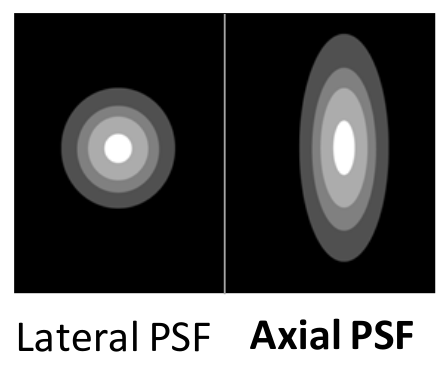
\includegraphics[width=0.3\linewidth]{./img/spim_01_psf.png}
			\caption{Une image des fonctions d'étalement de point (PSF) axiales et latérales en imagerie SPIM}
			\label{img:spim_01_point_spread_function}
		\end{figure}

		\begin{figure}[H]
			\centering
			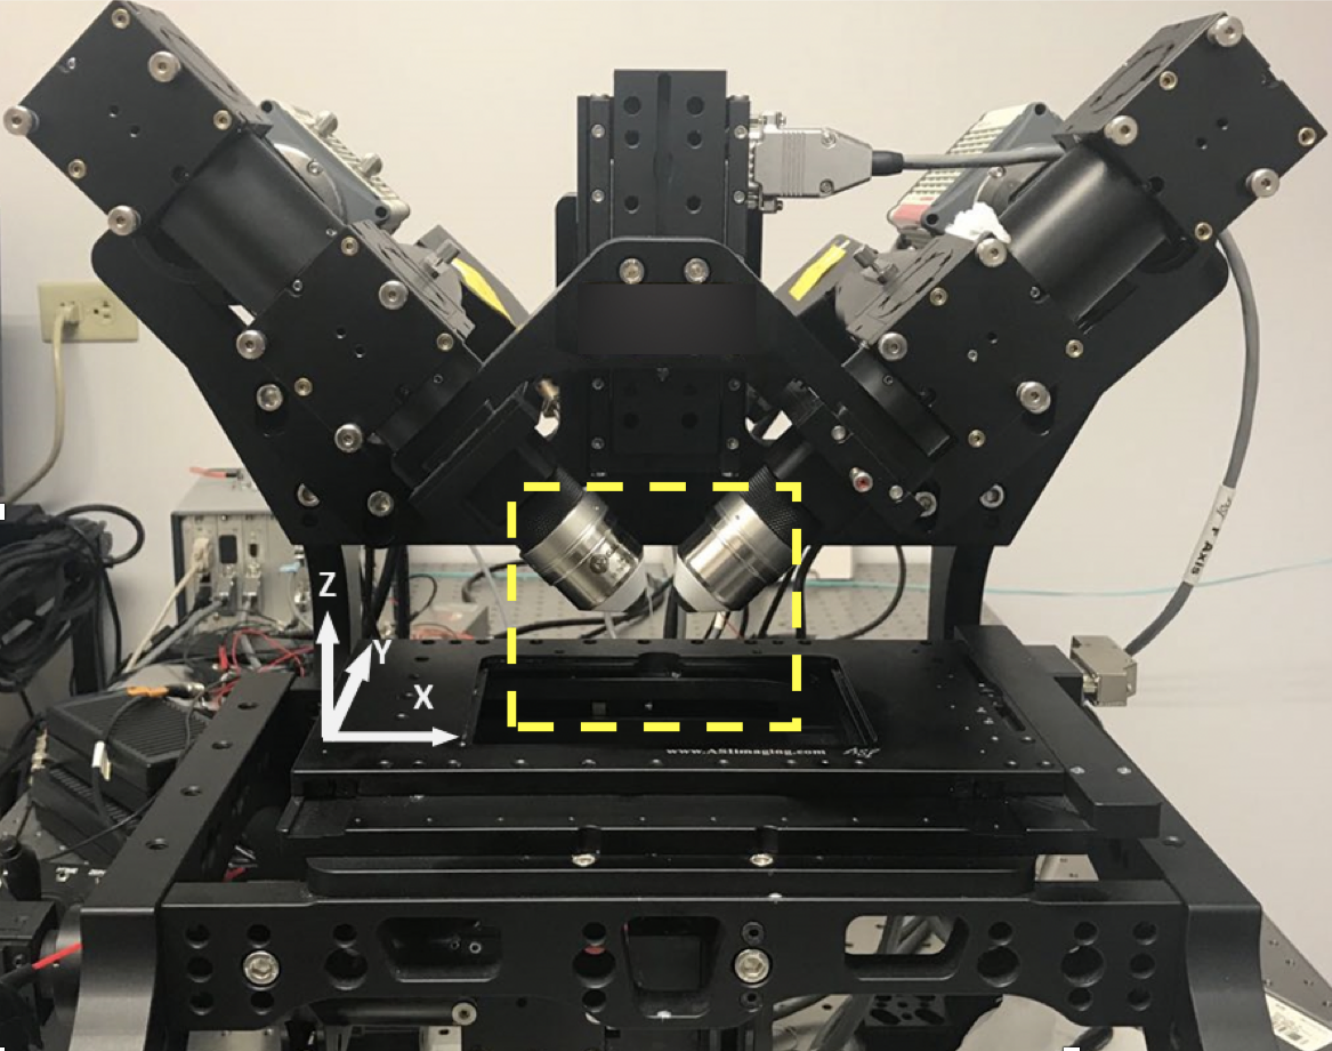
\includegraphics[width=0.5\linewidth]{./img/lsm_device_02.png}
			\caption{Le microscope \textit{diSPIM} conçu par les chercheurs de la Nouvelle Orléans permettant une acquisition tridimensionnelle d'un échantillon de manière fiable et rapide}
			\label{lsm_02_device}
		\end{figure}

		Dans cette méthode, il existe donc deux dispositifs \textit{SPIM} qui servent tour à tour de capteur, puis d'émetteur. Ces deux dispositifs sont placés à angle droit l'un de l'autre (voir \ref{lsm_02_device}), au dessus de la plateforme sur laquelle on dépose l'échantillon transparisé à analyser. Le fait d'avoir deux dispositifs \textit{SPIM} permet de se ramener à une acquisition 3D à résolution isotropique\footnotemark~ en combinant les acquisitions des capteurs avec leurs points de vue différents.\par
		\footnotetext{Inverse d'anisotropie : les propriétés sont les mêmes dans toutes directions}
	}
	% }}}

	%section gleason {{{
	\section{L'\'echelle de Gleason}
	{
		L'échelle de Gleason~\cite{cite_gleason_score} est une échelle pronostique\todo{Vocabulaire : Pronostiquable, qui permet de faire un pronostic ?} qui se base sur l'observation de la forme des cellules d'une prostate afin d'évaluer la possibilité de présence d'un cancer chez un patient. Inventée par Donald Gleason aux alentours de 1960, elle permet une évaluation fiable de la présence et, si présent, de l'avancement du développement d'un cancer de la prostate chez un individu. Cette échelle attribue un score de 1 à 5 en fonction de la forme des glandes ou cellules dans une coupe de la prostate.\par

		\commentaire{Insérer échelle ici, vue des différentes échelles de Gleason}\par

		Étant donné que cette échelle se base sur l'observation d'une seule coupe histologique de la prostate, la direction de la coupe, l'angle de celle-ci, son orientation ainsi que le type d'intersection avec la glande influera beaucoup la forme des glandes de la prostate et donc sur le pronostic final donné par un médecin après observation. Une des méthodes afin de pallier à cette incertitude, proposée par nos collaborateurs à la Nouvelle Orléans, serait d'analyser la morphologie tridimensionnelle des glandes. En effet, grâce à la méthode de microscopie \textit{di-SPIM}, nous pouvons obtenir une pile d'images permettant de reconstruire une grille volumique représentant l'échantillon acquis.\par

	}
	% }}}

	% section tulane {{{
	\section{Travaux réalisés par Tulane}
	{
		\commentaire{à dire : ils utilisent des outils non adaptés à la tâche (plugins ImageJ et code matlab non adapté), ne prennent pas en compte les spécificités du microscope qu'ils ont, et ensuite ils font meme pas les opérations prévues car prends trop de temps.}\par

		\commentaire{A parler aussi : les caractéristiques techniques du di-SPIM, et comment ils le prennent pas en compte}\par
	}
	% }}}

	\commentaire{avantage de nous amener à bord : on va reconstruire le modèle en prenant en compte les spécifiques de la diSpim qu'ils ont, faire tout à la volée pour réduire empreinte mémoire}\\
}

% VIM modeline : do not touch !
% vim: set spell spelllang=fr :
